\documentclass{article}

\usepackage{graphicx}
\usepackage{multirow}
\usepackage{amsmath,amssymb,amsfonts,amsthm, mathrsfs}
\usepackage[title]{appendix}
\usepackage{xcolor}
\usepackage{textcomp}
\usepackage{manyfoot, booktabs}
\usepackage{algorithm, algorithmicx, algpseudocode}
\usepackage{listings}
\usepackage{biblatex}

\usepackage[english]{babel}

\raggedbottom

\lstset{
    language=Python,                 
    basicstyle=\ttfamily\small,      
    keywordstyle=\color{blue},       
    stringstyle=\color{red},         
    commentstyle=\color{orange},      
    morecomment=[s][\color{gray}]{"""}{"""}, 
    numbers=left,                    
    numberstyle=\tiny\color{gray},   
    stepnumber=1,                    
    numbersep=10pt,                  
    backgroundcolor=\color{white},   
    showspaces=false,                
    showstringspaces=false,          
    showtabs=false,                  
    frame=single,                    
    captionpos=b,                    
    breaklines=true,                 
    breakatwhitespace=false,         
    tabsize=4,                       
    escapeinside={\%*}{*}           
}

\begin{document}

\title{F1 EDA - Big Data Final Term Project}

\author{Enrique Ulises Báez Gómez Tagle \\ Sara Rocío Miranda Mateos}

\maketitle

% MISSING \begin{abstract}% MISSING 

% MISSING \end{abstract}

\tableofcontents
\newpage

% MISSING \section{Introduction}% MISSING 


\section{Infrastructure / Architecture}

\begin{itemize}
    \item \textbf{Data Lakehouse Configuration:} Central to our project is a Data Lakehouse architecture designed for scalability and resilience within an AWS environment. This setup includes multiple layers of data storage and processing capabilities, ensuring efficient data management and analysis.
    
    \item \textbf{Storage Layers:} 
        \begin{itemize}
            \item \textbf{Raw Data Storage (RAW Layer):} Utilizes Amazon S3 to store unprocessed, raw data ingested from various sources.
            \item \textbf{Cleansed Data Storage (Cleansed Layer):} Stores cleaned and transformed data in Amazon S3, ready for further analysis.
            \item \textbf{Data Warehouse Storage (Data Warehouse Layer):} Contains structured and optimized data in Amazon S3, prepared for querying and visualization.
        \end{itemize}
    
    \item \textbf{Data Ingestion:} 
        \begin{itemize}
            \item \textbf{Real-Time Data Ingestion (AWS Lambda):} Handles the real-time ingestion of data, storing it in the RAW Layer.
            \item \textbf{Batch Data Ingestion (Static Dataset):} Manages the batch ingestion of static datasets, such as CSV files, into the RAW Layer.
        \end{itemize}
    
    \item \textbf{Data Transformation:} 
        \begin{itemize}
            \item \textbf{ETL Processing Jobs (AWS Glue):} Performs ETL (Extract, Transform, Load) operations to clean and transform data from the RAW Layer to the Cleansed Layer.
        \end{itemize}
    
    \item \textbf{Data Analysis:} 
        \begin{itemize}
            \item \textbf{Data Analytics and Processing (AWS EMR):} Utilizes Amazon EMR to run advanced data processing and analytical tasks on data from the Cleansed Layer, producing structured results stored in the Data Warehouse Layer.
        \end{itemize}
    
    \item \textbf{Data Cataloging:} 
        \begin{itemize}
            \item \textbf{Metadata Management (AWS Glue Data Catalog):} Catalogs the metadata of datasets in the Cleansed Layer, facilitating efficient data discovery and access.
        \end{itemize}
    
    \item \textbf{Data Visualization:} 
        \begin{itemize}
            \item \textbf{Visualization and Analysis (RStudio):} Processes the curated datasets in the Data Warehouse Layer locally to create insightful visualizations and analysis, supporting decision-making.
        \end{itemize}
    
    \item \textbf{Deployment Process:}
        \begin{enumerate}
            \item We initiated our deployment by setting up the AWS CLI, enabling us to interact with AWS services seamlessly.
            \item Amazon S3 buckets were created to host our data layers, carefully chosen to be in proximity to our compute resources to minimize latency.
            \item For infrastructure provisioning, we utilized both AWS CloudFormation and Terraform. AWS CloudFormation was used for managing AWS-specific resources, ensuring consistent and repeatable deployments within the AWS ecosystem. Terraform was employed for managing multi-cloud resources and ensuring infrastructure as code principles across various environments.
            \item AWS Glue was configured to automate our ETL processes, facilitating efficient data transformation and loading into our cleansed and data warehouse layers.
            \item Amazon EMR clusters were set up for big data processing, with configurations tailored to optimize performance and cost.
            \item Continuous Integration and Continuous Deployment (CI/CD) pipelines were implemented using AWS CodePipeline and Jenkins, automating the deployment process and ensuring that updates to our infrastructure and applications could be rolled out smoothly.
            \item Monitoring and logging were established using Amazon CloudWatch and AWS CloudTrail, providing real-time insights and audit trails for all activities within our environment.
            \item Security best practices were followed, including the use of IAM roles and policies to control access, as well as encryption of data at rest and in transit to protect our sensitive information.
        \end{enumerate}
    
\end{itemize}

This infrastructure is pivotal to our project, allowing us to effectively utilize big data technologies to derive valuable insights from the Formula 1 dataset. The design prioritizes scalability, efficiency, and cost-effectiveness, ensuring it meets the high demands of large-scale data processing and analysis. Ultimately, this setup empowers us to make data-driven decisions that enhance our understanding and strategic planning within the context of Formula 1.

\begin{figure}[H]
    \centering
    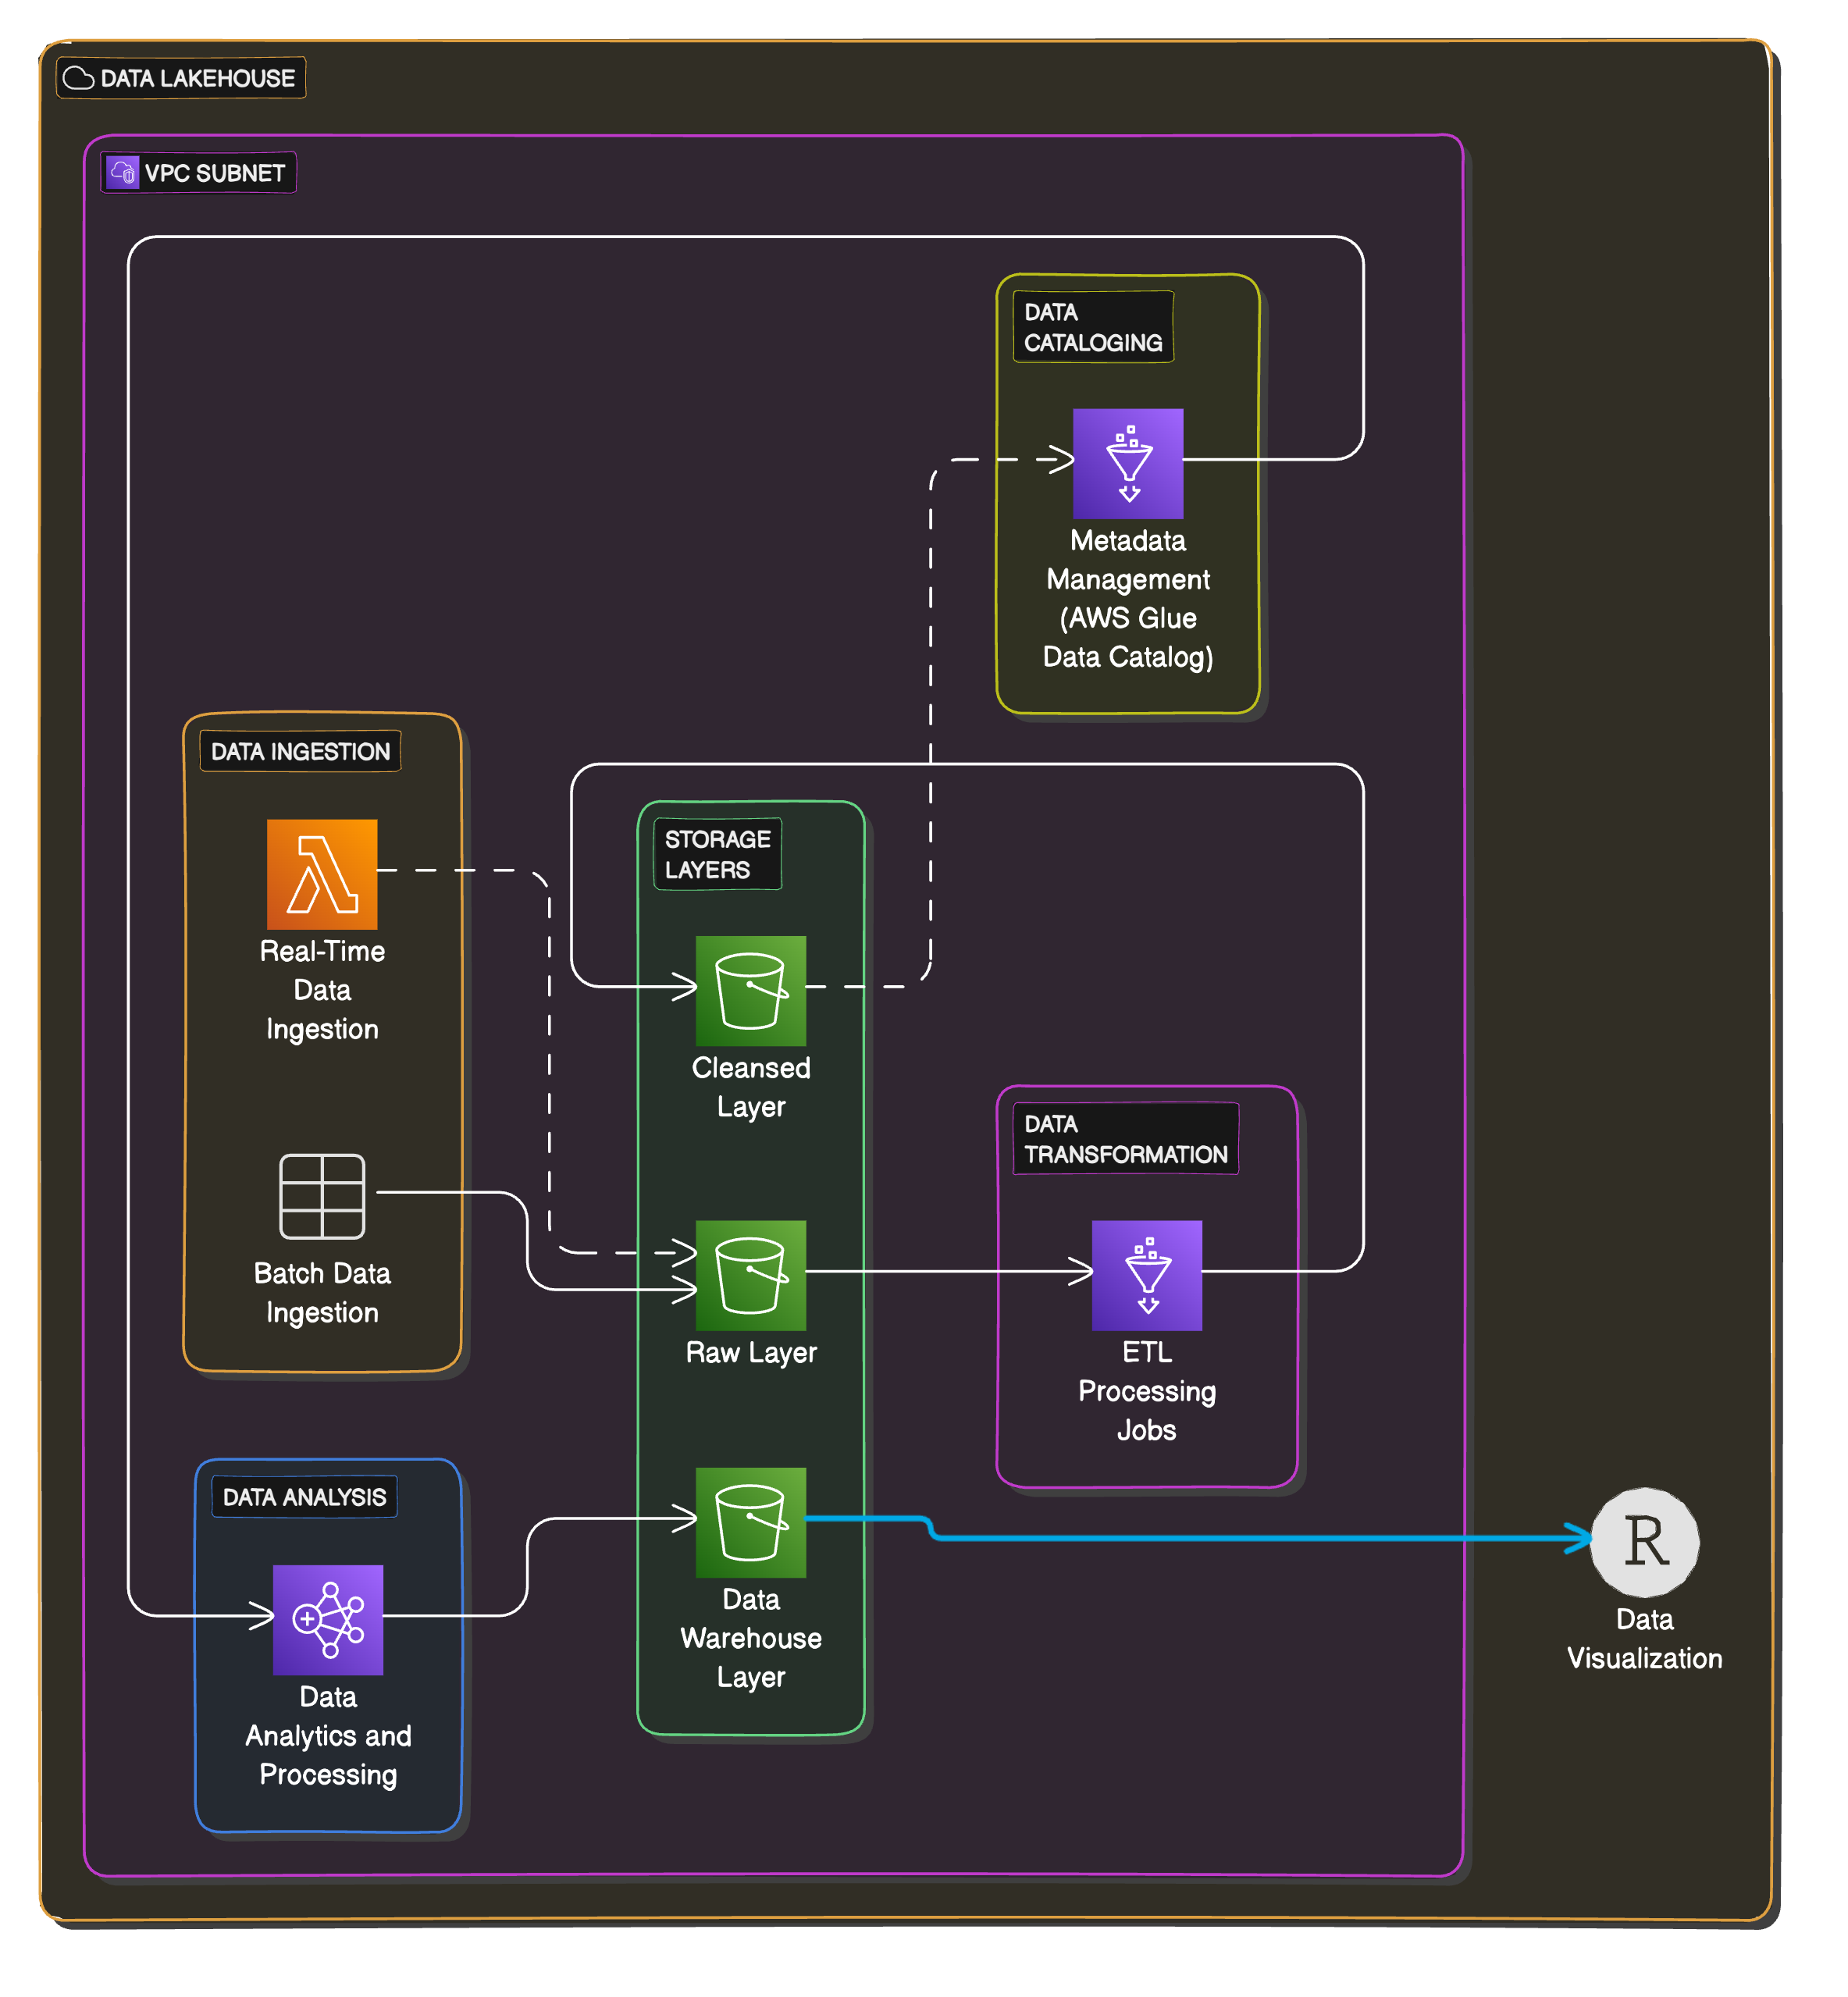
\includegraphics[width=0.7\textwidth]{images/arch/AWS-GridGuru-LakeHouseArchitecture.png}
    \caption{\textbf{AWS Data LakeHouse Architecture Diagram}}
\end{figure}

\section{Data Analysis with F1 Dataset}

We employed a dual dataset approach:

\begin{itemize}
    \item \textbf{Static Dataset:} This dataset contains historical information from past Formula 1 seasons. It includes data on race results, driver standings, lap times, and other relevant metrics.
    \item \textbf{Dynamic Dataset:} This dataset provides real-time information for the current 2024 season. AWS Lambda is used to ingest this data by making API calls to gather the latest updates, ensuring that our analysis remains current with ongoing events.
\end{itemize}
By integrating these datasets into our Data Lakehouse architecture on AWS, we effectively manage both historical and real-time data. The static dataset allows us to analyze trends and patterns over previous seasons, while the dynamic dataset enables us to monitor and react to live data from the current season.

Our analysis aimed to uncover actionable insights that could inform race strategies and enhance the performance of both teams and drivers. We utilized SQL queries on our Amazon EMR cluster to efficiently process and analyze the substantial data volumes. These queries were meticulously crafted to explore hypotheses regarding the relationships between various factors such as weather conditions, track characteristics, and driver performance metrics.

Upon obtaining initial results and drawing preliminary conclusions from these queries, we further refined our analysis by exporting the data to the Curated Layer in Amazon S3. These files were then imported into a dedicated workspace in RStudio for detailed visualization. This additional step allowed us to visually interpret the data more intuitively, facilitating the identification of significant patterns and trends that underpin our strategic recommendations.

\subsection{Database Structure Overview}
For our exploratory data analysis (EDA), we used a combination of historical and current datasets, structured into several tables with specific focuses. Each table captures unique aspects of the sport, allowing for a comprehensive analysis from multiple angles. Here's a brief guide to some tables:

\begin{itemize}
    \item \textbf{Circuits}: Contains details about the various circuits used in the races, including location, length, and other relevant information.
    \item \textbf{Constructor Results}: Records the results achieved by each constructor in different races, including points and status.
    \item \textbf{Constructor Standings}: Summarizes the standings of constructors throughout the season, capturing their cumulative points and positions.
    \item \textbf{Constructors}: Lists the constructors participating in a season, along with their basic information and attributes.
    \item \textbf{Driver Standings}: Details the standings of drivers across the season, showing their cumulative points and positions after each race.
    \item \textbf{Drivers}: Contains information about the drivers, including personal details, nationality, and career statistics.
    \item \textbf{Lap Times}: Records the times for each lap completed during race weekends, providing timing and performance data.
    \item \textbf{Pit Stops}: Details the pit stops made during races, including timing and duration.
    \item \textbf{Qualifying}: Captures the results of the qualifying sessions, determining the starting grid for the races.
    \item \textbf{Races}: Provides comprehensive information about each race event, including date, location, and participating drivers and constructors.
    \item \textbf{Results}: Summarizes the race results for each event, including positions, points, and other performance metrics.
    \item \textbf{Seasons}: Lists the seasons of the championship, including the year and other relevant details.
    \item \textbf{Sprint Results}: Contains the results of the sprint qualifying sessions, including grid positions and points awarded.
    \item \textbf{Status}: Describes the status of drivers in each race, such as whether they finished or the reason for not finishing.
\end{itemize}





\section{Challenges Encountered}
\subsection{Infrastructure-Related Challenges}
\paragraph{Description:}
Initially, our project was set up on Google Cloud Platform (GCP). However, we faced a significant challenge when our GCP credits were exhausted. To continue our work without interruption, we opted to create a simplified version of a Data Lakehouse on AWS. This decision was influenced by the opportunities and services available in AWS, which allowed us to replicate the necessary functionalities we initially had on GCP. We carefully selected AWS services that closely matched those we used on GCP to ensure a smooth transition and maintain the efficiency of our data processing and analysis.

% MISSING  \section{Conclusions} % MISSING 


\section{Project Repository}
\url{https://github.com/enriquegomeztagle/BigData/tree/main/FinalTerm/F1-GridGuru-Project}

\label{sec:references}
\begin{thebibliography}{9}
% \bibitem{ref1}

\end{thebibliography}

\end{document}
